% Intended LaTeX compiler: pdflatex
\documentclass[UTF8,a4paper,titlepage,10pt]{report}
\usepackage[utf8]{inputenc}
\usepackage[T1]{fontenc}
\usepackage{graphicx}
\usepackage{grffile}
\usepackage{longtable}
\usepackage{wrapfig}
\usepackage{rotating}
\usepackage[normalem]{ulem}
\usepackage{amsmath}
\usepackage{textcomp}
\usepackage{amssymb}
\usepackage{capt-of}
\usepackage{hyperref}
\usepackage[left=3.2cm,right=3.2cm,top=2.5cm,bottom=2.5cm]{geometry}
\hypersetup{colorlinks=true,linkcolor=blue}
\usepackage{tipa}
\usepackage[heading]{ctex}
\usepackage{rotfloat}
\usepackage{booktabs}
\usepackage{tabu}
\usepackage{enumitem}
\usepackage{makeidx}
\makeindex
\tabulinesep=1.0mm
\setlistdepth{9}
\renewlist{itemize}{itemize}{9}
\setlist[itemize]{label=$\circ$}
\author{winsphinX}
\date{}
\title{F.E.I.\\\medskip
\large Français \& Español \& Italiano}
\hypersetup{
 pdfauthor={winsphinX},
 pdftitle={F.E.I.},
 pdfkeywords={},
 pdfsubject={},
 pdfcreator={Emacs 27.2 (Org mode 9.4.6)},
 pdflang={English}}
\begin{document}

\maketitle
\tableofcontents

\part{序言}
\label{sec:org77cb5a9}

\chapter{简介}
\label{sec:orga538c1f}

\texttt{Français \& Español \& Italiano}

这三种语言同属 印欧语系-罗曼语族-西罗曼语支。

\begin{figure}[H]
\centering
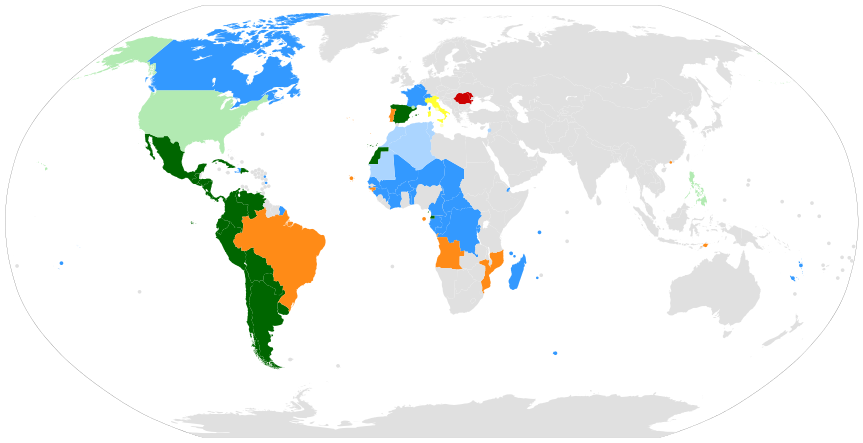
\includegraphics[width=0.9\textwidth]{images/WorldMap.png}
\caption{分布图}
\end{figure}

\section{发展}
\label{sec:orgd150aa5}

\begin{enumerate}
\item 演化
\label{sec:org45d85ca}

罗曼诸语言中使用者最多的是西班牙语,其后依次是葡萄牙语、法语、意大利语和罗马尼亚语。

在现代的罗曼诸语言中,拉丁语复杂的屈折变化和语法结构已经被大大简化。意大利语、萨丁尼亚语和古典拉丁语最接近。

在罗曼诸语言发展的历史中,最先从拉丁语中分裂出来成为独立语言的是萨丁尼亚語,随之而来的是东部的罗马尼亚语也与拉丁语脱离,成为独立语言。第三个重要过程是意大利语与高卢-伊比利亚语言的分离。这个时候,法国和伊比利亚半岛诸国的语言仍然具有高度的一致性。罗曼语言的第四次重大变化是伊比利亚半岛的语言和法语脱离,逐渐形成非常相似的两种现代语言:西班牙语和葡萄牙语。而通行于西班牙东部的加泰罗尼亚语则被认为是法语和伊比利亚语言的中间产物,因为这种语言融合了法语和西、葡两种语言的很多特征。

\begin{figure}[H]
\centering
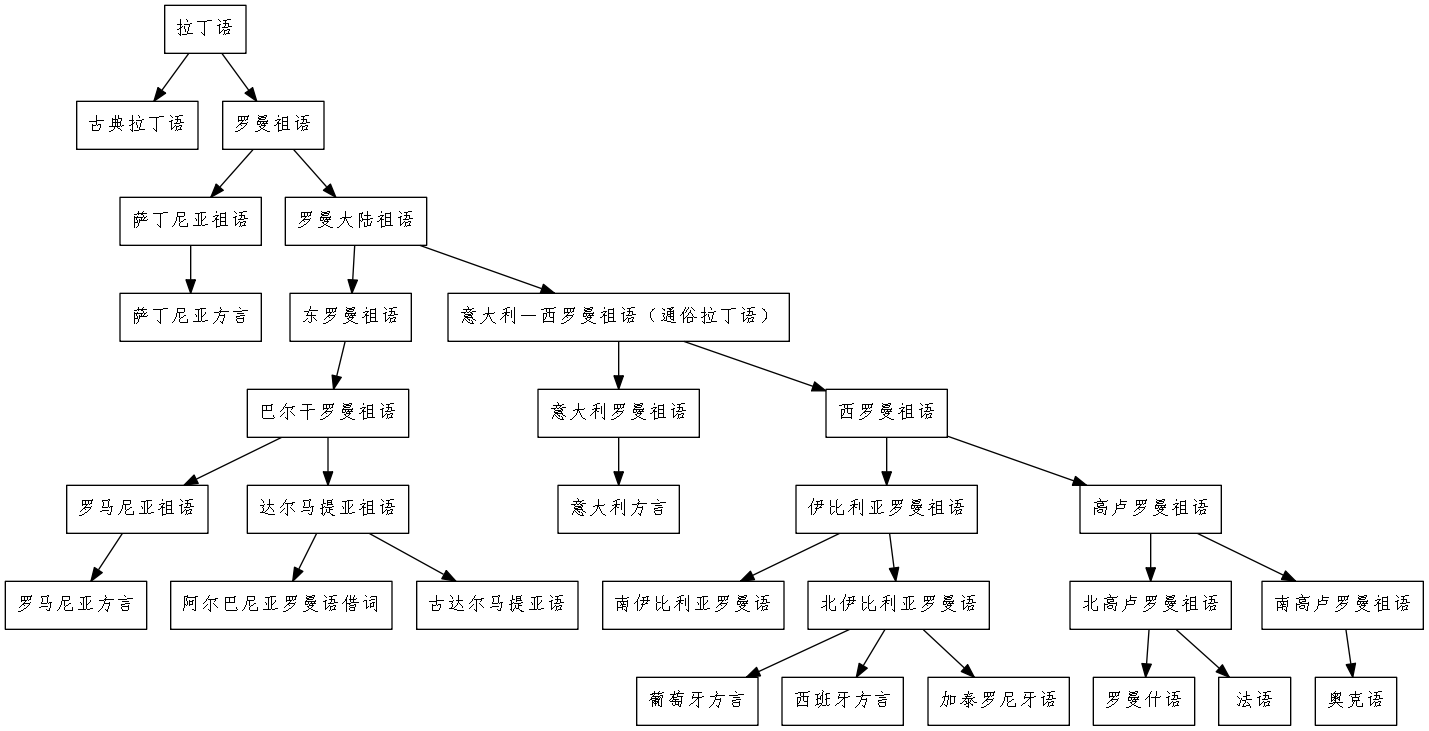
\includegraphics[width=0.9\textwidth]{images/FamilyMap.png}
\caption{演化图}
\end{figure}

\item 分支
\label{sec:org032c797}

\begin{itemize}
\item 东罗曼语支
\begin{itemize}
\item 罗马尼亚语 (ron)
\item 伊斯特拉-罗马尼亚语(Romanian, Istro)(ruo)
\item 阿罗马尼亚语、马其顿-罗马尼亚语(Romanian, Macedo)(rup)
\item 梅戈来诺-罗马尼亚语(Romanian, Megleno)(ruq)
\end{itemize}
\item 意大利-西罗曼语支
\begin{itemize}
\item 意大利-达尔马提亚语支
\begin{itemize}
\item 达尔马提亚语(Dalmatian)(dlm)(已灭绝)
\item 伊斯特拉语(Istriot)(ist)
\item 意大利语 (ita)
\item 犹太-意大利语(Judeo-Italian)(itk)
\item 拿坡里语 (nap)
\item 西西里语 (scn)
\item 科西嘉语 Corsican(cos)(一说属于南罗曼语支)
\end{itemize}
\item 西罗曼语支
\begin{itemize}
\item 高卢-意大利语支 Gallo-Italian
\begin{itemize}
\item 艾米利亚-罗马涅语(Emiliano-Romagnolo)(eml)
\item 利古里亚语(Ligurian)(lij)
\item 伦巴底语 (lmo)
\item 皮埃蒙特语 (pms)
\item 威尼斯语 (vec)
\end{itemize}
\item 高卢-罗曼语支 Gallo-Romance
\begin{itemize}
\item 奥依语
\begin{itemize}
\item 法语
\begin{itemize}
\item 古法语 (fro)
\item 盎格鲁-诺曼语 (xno)
\item 法语 (fra)
\item 卡真法语、路易斯安那州法语(Cajun French)(frc)
\item 庇卡底语(Picard)(pcd)
\item 瓦龙语、瓦隆语、华隆语(Wallon)(wln)
\item 查法蒂语、犹太-法语(Zarphatic)(zrp)
\end{itemize}
\end{itemize}
\item 东南奥依语
\begin{itemize}
\item 法兰克-普罗旺斯语(Franco-Provençal)(frp)
\end{itemize}
\item 雷蒂亚-罗曼语(Rhaeto-Romance)
\begin{itemize}
\item 弗留利语 (fur)
\item 拉登语 (lld)
\item 罗曼什语 (roh)
\end{itemize}
\item 奥克-罗曼语(一说属于伊比利亚-罗曼语支下的东伊比利亚语支)
\begin{itemize}
\item 奥克语 (oci)
\item 古普罗旺斯语(Old Provençal)(pro)
\item 苏阿迪特语(Shuadit)(sdt)
\item 加泰罗尼亚语、瓦伦西亚语 (cat)
\end{itemize}
\end{itemize}
\item 伊比利亚-罗曼语支 Ibero-Romance
\begin{itemize}
\item 西伊比利亚语支 West Iberian
\begin{itemize}
\item Asturo-Leonese
\begin{itemize}
\item 阿斯图里亚斯语 (ast)
\item 米兰德斯语(Miranda do Douro)(mwl)
\end{itemize}
\item 卡斯提语 Castilian
\begin{itemize}
\item 埃斯特雷马杜拉语(Extremaduran)(ext)
\item 拉迪诺语、犹太-西班牙语 (lad)
\item 西班牙语 (spa)
\item 洛雷托-乌卡亚利西班牙语、森林西班牙语(Spanish, Loreto-Ucayali,在秘鲁)(spq)
\end{itemize}
\end{itemize}
\end{itemize}
\item 葡萄牙-加利西亚 Portuguese-Galician
\begin{itemize}
\item 法拉语(Fala)(fax)
\item 加利西亚语 (glg)
\item 葡萄牙语 (por)
\end{itemize}
\item 比利牛斯-莫札拉布语支 Pyrenean-Mozarabic
\begin{itemize}
\item 莫札拉布语(Mozarabic)(mxi)
\item 阿拉贡语 (arg)
\end{itemize}
\end{itemize}
\item 南罗曼语支(海岛语支)
\begin{itemize}
\item 古科西嘉语
\item 萨丁尼亚语(Sardinian)(srd)
\begin{itemize}
\item 萨萨里方言(Sardinian, Sassarese)(sdc)
\item 加卢拉方言(Sardinian, Gallurese)(sdn)
\item 劳古多罗方言(Sardinian, Logudorese)(src)
\item 坎皮达诺方言(Sardinian, Campidanese)(sro)
\end{itemize}
\end{itemize}
\end{itemize}
\end{itemize}
\end{enumerate}

\section{比较}
\label{sec:org8e2707c}

\begin{enumerate}
\item 共同点
\label{sec:org2b2131a}

\begin{itemize}
\item 语法上:
\begin{itemize}
\item 对动作的描述更多的依赖动词自身的变化。语法变化主要依靠动词的词形变化,而非依靠粘着成分。这也是罗曼语言构词法的重要特征。
\item 通常频繁使用两个助动词来构成时态,都是从拉丁语的不定词 esse 和 stare 改变而来的,一个用于描述本质,一个用于描述状态。
\item 动词都要依照人称及数量的不同而进行变位。第三人称通常有语法性的区别,而第一和第二人称则没有。
\item 保留着敬词的痕迹,主要体现在第二人称单数上。
\item 名词都有语法性的区别,但通常只有两种语法性,而拉丁语中名词则有三个语法性。
\item 除罗马尼亚语之外,其他语言已经没有格变化。多以冠词和介词来替代拉丁语词尾复杂的格变化。
\end{itemize}
\item 语音上:
\begin{itemize}
\item 在语音上,通常都将每个词的重音放在倒数第二个音节上(在法语中,重音是放在最后一个音节上的,因为多数法语词汇摈弃了语言词汇的最后一个元音)。
\item 通常都有一些特殊的规定以消除声门塞音、闭塞辅音等对语言整体美感的影响(例如法语中就有“联诵”的规定)。这些特征使得所有的罗曼语言都具有语速快、语调流畅的特点。
\end{itemize}
\item 书写上:
\begin{itemize}
\item 字母 W 和 K 使用得很少,通常只出现在人名和外来语中。
\item 字母 C 和 G 在前元音(如 i、e 等)之前的时候通常读音要软化,在后元音(如 a、o、u)前则要发较硬的软腭音。
\item 一些表示国籍的形容词、表示星期、月份和年份的名词通常首字母不需大写。
\end{itemize}
\end{itemize}

\item 差异点
\label{sec:org8db52bd}

\begin{itemize}
\item 在一些罗曼语中,名词复数是由名词单数词尾加字母 s 构成的,这是从拉丁语中宾格名词的复数形式演化而来的,以这种方式构成名词复数的罗曼语言包括葡萄牙语、西班牙语、加泰罗尼亚语、普罗旺斯语和法语。也有一些语言的名词复数是由词尾的元音字母变化而构成的,这一特征则是从拉丁语中主格名词的复数形式演化而来。如意大利语和罗马尼亚语等。
\item 一些罗曼语言摈弃了语言词汇的词尾非重读元音。例如欧洲语言的词汇月亮在意大利语中仍是 luna,而在法语中则变成了 lune。仍然保留了词尾元音的语言包括葡萄牙语、西班牙语、意大利语和罗马尼亚语。而法语则摈弃了词尾元音。
\item 罗曼诸语言的比较级构成词也有两种,一种是使用 plus 一词的,一种则是使用 magis 一词的。采用前一种构成方式的语言包括法语(plus)和意大利语(più);而采用后一种构成方式的则包括葡萄牙语(mais)、西班牙语(más)、加泰罗尼亚语(més)等。
\item 在罗曼语言中,“16”这个数字在计数体系中地位非常特殊。除了罗马尼亚语以外,罗曼语言普遍用“1+10”,“2+10”……结构表示 11-15,用“10+7”,“10+8”……结构表示 17-19。而 16 作为两组之间的分界线,在各语言中表达方法不同,其中法语、加泰罗尼亚语、意大利语等用“6+10”表示;而葡萄牙语和西班牙语等则用“10+6”表示。
\item 有些罗曼语言用表达“有”这一含义的助动词来构成复合时态(比如法语中的“愈过去时”等),而有些语言则对动词做出区分,有些动词用“有”来构成,有些则要用“是”来构成。仅使用“有”构成的语言包括加泰罗尼亚语、葡萄牙语、西班牙语和罗马尼亚语等。而混合使用两个助动词的语言则包括法语、意大利语和普罗旺斯语等。在后一类罗曼语言中,用“是”来构成的复合时态的动词通常是常用的不及物动词,这类动词通常描述的是无法确定目标或标明状态的动作。例如“来”、“去”、“变为”等等。而大多数动词还是要利用“有”来构成复合时态。
\end{itemize}
\end{enumerate}

\chapter{辨识}
\label{sec:org2d8c9e5}

\begin{itemize}
\item \textbf{一看}
\begin{itemize}
\item c 下面带勾的(ç)一定是法语;n 上面带波浪的(ñ),有特殊标点的(问号 ¿?、叹号 ¡!)一定是西班牙语;双辅音较多的一定是意大利语。
\item 元音上面只有左撇的(闭音符),一定是西班牙语;同时有左撇和右撇(开音符)的,是意大利语;不但有左撇和右撇,还有帽子(长音符)的,一定是法语。
\end{itemize}
\item \textbf{二听}
\begin{itemize}
\item 带小舌颤音的一定是法语;发音有很多 -s 的一定是西班牙语;腔调比较特别的是意大利语。
\end{itemize}
\end{itemize}

\part{语音}
\label{sec:org6256edc}

\chapter{字母}
\label{sec:org4c35a20}

\section{字母表}
\label{sec:org174b71a}
\begin{enumerate}
\item Français
\label{sec:org148ccde}

\begin{longtabu} to 0.9\textwidth {XXX|XXX}
\caption{法语字母表}
\\
\toprule
字母 & 名称 & 读音 & 字母 & 名称 & 读音\\
\midrule
\endfirsthead
\multicolumn{6}{l}{Continued from previous page} \\
\toprule

字母 & 名称 & 读音 & 字母 & 名称 & 读音 \\

\midrule
\endhead
\midrule\multicolumn{6}{r}{Continued on next page} \\
\endfoot
\endlastfoot
A a & a & \textipa{[A]} & N n & enne & \textipa{[En]}\\
B b & bé & \textipa{[be]} & O o & o & \textipa{[o]}\\
C c & cé & \textipa{[se]} & P p & pé & \textipa{[pe]}\\
D d & dé & \textipa{[de]} & Q q & qu & \textipa{[ky]}\\
E e & e & \textipa{[@]} & R r & erre & \textipa{[E:K]}\\
F e & eff & \textipa{[Ef]} & S s & esse & \textipa{[Es]}\\
G g & gé & \textipa{[Ze]} & T t & té & \textipa{[te]}\\
H h & hache & \textipa{[AS]} & U u & u & \textipa{[y]}\\
I i & i & \textipa{[i]} & V v & vé & \textipa{[ve]}\\
J j & ji & \textipa{[Zi]} & W w & double vé & \textipa{[dubl@ve]}\\
K k & ka & \textipa{[kA]} & X x & ixe & \textipa{[iks]}\\
L l & elle & \textipa{[El]} & Y y & i grec & \textipa{[igKEk]}\\
M m & emme & \textipa{[Em]} & Z z & zède & \textipa{[zEd]}\\
\bottomrule
\end{longtabu}

\item Español
\label{sec:org66a3a33}

\begin{longtabu} to 0.9\textwidth {XXX|XXX}
\caption{西班牙语字母表}
\\
\toprule
字母 & 名称 & 读音 & 字母 & 名称 & 读音\\
\midrule
\endfirsthead
\multicolumn{6}{l}{Continued from previous page} \\
\toprule

字母 & 名称 & 读音 & 字母 & 名称 & 读音 \\

\midrule
\endhead
\midrule\multicolumn{6}{r}{Continued on next page} \\
\endfoot
\endlastfoot
A a & a & \textipa{[A]} & N n & ene & \textipa{[ene]}\\
B b & be & \textipa{[be]} & Ñ ñ & eñe & \textipa{[e\textltailn e]}\\
C c & ce & \textipa{[Te]} & O o & o & \textipa{[o]}\\
CH ch & che & \textipa{[tSe]} & P p & pe & \textipa{[pe]}\\
D d & de & \textipa{[de]} & Q q & cu & \textipa{[ku]}\\
E e & e & \textipa{[e]} & R r & ere & \textipa{[eRe]}\\
F e & efe & \textipa{[efe]} & RR rr & erre & \textipa{[ere]}\\
G g & ge & \textipa{[xe]} & S s & ese & \textipa{[ese]}\\
H h & hache & \textipa{[AtSe]} & T t & te & \textipa{[te]}\\
I i & i & \textipa{[i]} & U u & u & \textipa{[u]}\\
J j & jota & \textipa{[xotA]} & V v & uve & \textipa{[uBe]}\\
K k & ca & \textipa{[kA]} & W w & uve doble & \textipa{[uBedoBle]}\\
L l & ele & \textipa{[ele]} & X x & equis & \textipa{[ekis]}\\
LL ll & elle & \textipa{[eJe]} & Y y & i griega & \textipa{[igriegA]}\\
M m & eme & \textipa{[eme]} & Z z & zeta & \textipa{[Teta]}\\
\bottomrule
\end{longtabu}

\begin{itemize}
\item 在西班牙语中,字母 ``K'' 和 ``W'' 平常时一般不用,它们只出现于外来词汇。
\end{itemize}

\item Italiano
\label{sec:org27ca4e9}

\begin{longtabu} to 0.9\textwidth {XXX|XXX}
\caption{意大利语字母表}
\\
\toprule
字母 & 名称 & 读音 & 字母 & 名称 & 读音\\
\midrule
\endfirsthead
\multicolumn{6}{l}{Continued from previous page} \\
\toprule

字母 & 名称 & 读音 & 字母 & 名称 & 读音 \\

\midrule
\endhead
\midrule\multicolumn{6}{r}{Continued on next page} \\
\endfoot
\endlastfoot
A a & a & \textipa{[A]} & N n & enne & \textipa{[enne]}\\
B b & bi & \textipa{[bi]} & O o & o & \textipa{[o]}\\
C c & ci & \textipa{[tSi]} & P p & pi & \textipa{[pi]}\\
D d & di & \textipa{[di]} & Q q & cu & \textipa{[ku]}\\
E e & e & \textipa{[e]} & R r & erre & \textipa{[erre]}\\
F e & effe & \textipa{[effe]} & S s & esse & \textipa{[esse]}\\
G g & gi & \textipa{[dZi]} & T t & ti & \textipa{[ti]}\\
H h & acca & \textipa{[AkkA]} & U u & u & \textipa{[u]}\\
I i & i & \textipa{[i]} & V v & vu & \textipa{[vu]}\\
J j & i lungo & \textipa{[ilungo]} & W w & doppia vu & \textipa{[doppiAvu]}\\
K k & cappa & \textipa{[kAppA]} & X x & ics & \textipa{[iks]}\\
L l & elle & \textipa{[elle]} & Y y & ipsilon & \textipa{[ipsilon]}\\
M m & emme & \textipa{[emme]} & Z z & zeta & \textipa{[tseta]}\\
\bottomrule
\end{longtabu}

\begin{itemize}
\item 在意大利语中,字母 ``J''、``K''、``W''、``X''、``Y'' 只用于外来词汇。
\end{itemize}
\end{enumerate}

\section{音符表}
\label{sec:orgdc714da}

\begin{longtabu} to 0.9\textwidth {X|X|X|X}
\caption{音符汇总表}
\\
\toprule
音符名 & 法语适用字母 & 西班牙语适用字母 & 意大利语适用字母\\
\midrule
\endfirsthead
\multicolumn{4}{l}{Continued from previous page} \\
\toprule

音符名 & 法语适用字母 & 西班牙语适用字母 & 意大利语适用字母 \\

\midrule
\endhead
\midrule\multicolumn{4}{r}{Continued on next page} \\
\endfoot
\endlastfoot
闭音符 & é & á, é, í, ó, ú, ý & é, ó\\
开音符 & à, è, ù & - & à, è, ì, ò\\
长音符 & â, ê, î, ô, û & - & -\\
分音符 & ë, ï, ü, ÿ & ï, ü & -\\
软音符 & ç & - & -\\
颚化符 & - & ñ & -\\
\bottomrule
\end{longtabu}

\chapter{发音}
\label{sec:org7ff840e}

\section{发音总表}
\label{sec:orge26edfc}

\begin{longtabu} to 0.9\textwidth {l|X|X|X}
\caption{元音汇总表}
\\
\toprule
音标 & 法语 & 西班牙语 & 意大利语\\
\midrule
\endfirsthead
\multicolumn{4}{l}{Continued from previous page} \\
\toprule

音标 & 法语 & 西班牙语 & 意大利语 \\

\midrule
\endhead
\midrule\multicolumn{4}{r}{Continued on next page} \\
\endfoot
\endlastfoot
\textipa{[A]} & a, à, â & a & a, à\\
\textipa{[E]} & è, ê, ë, ai, aî, ei, -et & e & è\\
\textipa{[e]} & é, -er, -ez, -ed, es- & - & e, é\\
\textipa{[i]} & i, î, ï & i & i, ì, í\\
\textipa{[O]} & o, au[r], & - & ò\\
\textipa{[o]} & o, ô, o[z], au, eau & o & o, ó\\
\textipa{[u]} & ou, où, oû & u & u, ù, ú\\
\textipa{[y]} & u, û & - & -\\
\textipa{[@]} & e & - & -\\
\textipa{[\o]} & eu, œu, eu[zdt] & - & -\\
\textipa{[\oe]} & eu, œu, [cg]ue, œ & - & -\\
\textipa{[\~E]} & in, im, yn, ym, ain, aim, ein, un, um & - & -\\
\textipa{[\~A]} & an, am, en, em & - & -\\
\textipa{[\~O]} & on, om & - & -\\
\bottomrule
\end{longtabu}

\begin{longtabu} to 0.9\textwidth {l|X|X|X}
\caption{辅音汇总表}
\\
\toprule
音标 & 法语 & 西班牙语 & 意大利语\\
\midrule
\endfirsthead
\multicolumn{4}{l}{Continued from previous page} \\
\toprule

音标 & 法语 & 西班牙语 & 意大利语 \\

\midrule
\endhead
\midrule\multicolumn{4}{r}{Continued on next page} \\
\endfoot
\endlastfoot
\textipa{[p]} & p & p & p\\
\textipa{[b]} & b & b-, v- & b\\
\textipa{[B]} & - & -b, -v & -\\
\midrule
\textipa{[t]} & t & t & t\\
\textipa{[d]} & d & d- & d\\
\textipa{[D]} & - & -d- & -\\
\textipa{[T]} & - & -d, z, c-ei & -\\
\midrule
\textipa{[k]} & c-aou, k, ck, qu, -q & c-aou, qu-ei & c-aou, ch-ei\\
\textipa{[g]} & g-aou, gu-eiy & g-aou, gu-ei & g-aou, gh-ei\\
\textipa{[x]} & - & j, g-ei & -\\
\midrule
\textipa{[s]} & s, ss, c-eiy, ç, x & s, x & s\\
\textipa{[z]} & z, zz, -s-, x & - & -s-\\
\midrule
\textipa{[f]} & f, ff, ph & f & f\\
\textipa{[v]} & v & - & v\\
\midrule
\textipa{[S]} & ch & - & sc-ei\\
\textipa{[Z]} & j, g-eiy & - & -\\
\midrule
\textipa{[tS]} & - & ch & c-ei\\
\textipa{[dZ]} & - & - & g-ei\\
\midrule
\textipa{[ts]} & - & - & z\\
\textipa{[dz]} & - & - & z\\
\midrule
\textipa{[m]} & m & m & m\\
\textipa{[n]} & n & n & n\\
\textipa{[\textltailn]} & gn & ñ & gn\\
\textipa{[l]} & l & l & l\\
\textipa{[L]} & - & - & gli\\
\textipa{[J]} & - & ll, y- & -\\
\textipa{[r]} & - & rr & r\\
\textipa{[R]} & - & r & -\\
\textipa{[K]} & r & - & -\\
\midrule
\textipa{[j]} & i-, -il, -ill, y- & i- & i-\\
\textipa{[w]} & ou-, w & u-, w & u-, w\\
\textipa{[4]} & u- & - & -\\
\bottomrule
\end{longtabu}

\section{发音规则}
\label{sec:org20f6382}

\begin{enumerate}
\item Français
\label{sec:orgf036b94}

\begin{longtabu} to 0.9\textwidth {X|l|X}
\caption{法语元音表}
\\
\toprule
字母组合 & 读音 & 例词\\
\midrule
\endfirsthead
\multicolumn{3}{l}{Continued from previous page} \\
\toprule

字母组合 & 读音 & 例词 \\

\midrule
\endhead
\midrule\multicolumn{3}{r}{Continued on next page} \\
\endfoot
\endlastfoot
a, à, â & \textipa{[A]} & banane, là, fâché\\
e 在 mm 或 nn 前(少数词) &  & femme, solennel\\
\midrule
è, ê, ë & \textipa{[E]} & mère, fête, noël\\
ai, aî, ei &  & lait, maître, reine\\
e 在闭音节中 &  & mer, service, respect\\
e 在两个相同的辅音字母前(m, n 除外) &  & belle, cette, adresse\\
-et 在词末 &  & poulet, filet\\
\midrule
é & \textipa{[e]} & été, léger\\
-er, -ez, -ed 在词尾 &  & loger, visiter, parler, chez, pied\\
es 在单音节词中 &  & les, des, ces\\
ess-, eff-, desc-, dess- 在词首 &  & essai, effet, descendre, dessert\\
\midrule
i, î, ï 及 y & \textipa{[i]} & petit, finir, île, maïs, bicyclette\\
\midrule
u 和 û & \textipa{[y]} & tu, but, flûte, sûr, culture\\
\midrule
ou,où,oû & \textipa{[u]} & loup, où, coût\\
\midrule
ô & \textipa{[o]} & tôt, allô\\
o 在\textipa{[z]}音前 &  & chose, rose\\
o 在词末开音节中 &  & vélo, mot\\
au &  & chaud, cause\\
eau &  & beau, bureau\\
\midrule
o 除发\textipa{[o]}音的情况以外 & \textipa{[O]} & robe, porte, photo\\
au 在 r 前 &  & aurore, aurai\\
\midrule
e 在单音节词中 & \textipa{[@]} & le, te, de, ce\\
e 在词首开音节中 &  & venir, lever, demain\\
e 在“辅辅-e-辅”结构中 &  & entreprise, mercredi, partenaire\\
\midrule
eu, œu 在词末开音节中 & \textipa{[\o]} & peu, deux, vœu, nœud\\
eu 在\textipa{[z]}前 &  & heureuse, vendeuse\\
eu 在\textipa{[d][t][tr]}前 &  & jeudi, émeute, neutre\\
\midrule
eu, œu 除了发\textipa{[\o]}音的情况以外 & \textipa{[\oe]} & fleur, peur, seuil, sœur\\
ue 在 c, g 后 &  & accueil, orgueil\\
œ 在少数单词中 &  & œil\\
\midrule
im, in, ym, yn, aim, ain, ein, um, un(后面不是元音或 m, n) & \textipa{[\~E]} & fin, timbre, syndicat, symbole, faim, pain, plein, lundi, commun\\
\midrule
am, an, em, en(后面不是元音或 m, n) & \textipa{[\~A]} & chambre, champagne, ancre, chanter, emporter, remplir, entrer, content\\
\midrule
om, on(后面不是元音或 m, n) & \textipa{[\~O]} & ombre, tomber, rompre, oncle, salon, chanson\\
\bottomrule
\end{longtabu}

\begin{itemize}
\item 字母组合 um, un,其发音\textipa{[\~\oe]},已有被\textipa{[\~E]}替代的趋势。
\end{itemize}

\begin{longtabu} to 0.9\textwidth {X|l|X}
\caption{法语辅音表}
\\
\toprule
字母组合 & 读音 & 例词\\
\midrule
\endfirsthead
\multicolumn{3}{l}{Continued from previous page} \\
\toprule

字母组合 & 读音 & 例词 \\

\midrule
\endhead
\midrule\multicolumn{3}{r}{Continued on next page} \\
\endfoot
\endlastfoot
p, pp & \textipa{[p]} & pape, impact, palace, parc, Philippe, pratique\\
b, bb & \textipa{[b]} & banque, bicyclette, herbe, abbé, Bible\\
\midrule
t, tt & \textipa{[t]} & tête, table, thé, patte, maître\\
d, dd & \textipa{[d]} & madame, date, déjà, addition, adresse\\
\midrule
k, ck & \textipa{[k]} & kilo, ticket\\
c 在 a, o, u, 辅音字母前或词末 & \textipa{[k]} & casser, coller, cube, clé, lac\\
qu & \textipa{[k]} & tonique, qui, quel\\
q 在词末 & \textipa{[k]} & coq, cinq\\
g 在 a, o, u 及辅音字母前 & \textipa{[g]} & gare, goûter, figure, jungle\\
gu 在 e, i, y 前 & \textipa{[g]} & guetter, guide, Guy\\
\midrule
s, ss & \textipa{[s]} & veste, système,adresse, messe\\
c 在 e, i, y 前 & \textipa{[s]} & cinéma, cycle, scientifique, centre\\
ç & \textipa{[s]} & français, leçon\\
t 在 tion 和 tie 中(前面没有 s) & \textipa{[s]} & attention, nation, démocratie, patience\\
x 在少数词中 & \textipa{[s]} & dix, six\\
z, zz & \textipa{[z]} & gaz, seize, zéro, jazz\\
s 在两个元音字母之间 & \textipa{[z]} & base, visage, paisible\\
x 在个别词中 & \textipa{[z]} & deuxième, sixième\\
\midrule
ch & \textipa{[S]} & Chine, douche\\
j & \textipa{[Z]} & je, jour\\
g 在 e, i, y 前 & \textipa{[Z]} & geste, gilet, gymnastique\\
\midrule
f, ff, ph & \textipa{[f]} & flamme, difficile, chef, philosophie\\
v & \textipa{[v]} & veste, vivre, voir\\
\midrule
l & \textipa{[l]} & loi, facile, allocution, fil, cil\\
m & \textipa{[m]} & ma, pomme, image, mythe\\
n, nn & \textipa{[n]} & minute, année\\
mn 在少数单词中 & \textipa{[n]} & condamner, automne\\
gn & \textipa{[\textltailn]} & signe, campagne, gagner, magnifique, digne\\
r, rr & \textipa{[K]} & rare, mer, gris, bracelet, prune, crèche, Méditerranée\\
\midrule
ou 在元音前 & \textipa{[w]} & jouer, mouette, oui, souhait\\
w 在少数外来词中 & \textipa{[w]} & watt\\
\midrule
i 在元音前 & \textipa{[j]} & lien, ciel, faïence\\
il 在词末且在元音后 & \textipa{[j]} & réveil, travail\\
ill 在元音后 & \textipa{[j]} & bataille, travailler\\
字母 y 在元音前或在词首 & \textipa{[j]} & Lyon, yeux\\
\midrule
u 在元音前 & \textipa{[4]} & nuit lui, fruit, juin\\
\bottomrule
\end{longtabu}

\begin{itemize}
\item 除联诵时,词尾的 d, g, p, s, t, x 和 z 一般不发音。
\end{itemize}

\item Español
\label{sec:orga8645c0}

\begin{longtabu} to 0.9\textwidth {X|l|X}
\caption{西班牙语元音表}
\\
\toprule
字母组合 & 读音 & 例词\\
\midrule
\endfirsthead
\multicolumn{3}{l}{Continued from previous page} \\
\toprule

字母组合 & 读音 & 例词 \\

\midrule
\endhead
\midrule\multicolumn{3}{r}{Continued on next page} \\
\endfoot
\endlastfoot
a & \textipa{[A]} & ala, amigo\\
e & \textipa{[E]} & eco, esta\\
i & \textipa{[i]} & idea, isla\\
o & \textipa{[o]} & oso, solo\\
u & \textipa{[u]} & uva, luz\\
\midrule
ai, ay & \textipa{[Ai]} & aire, hay\\
ei, ey & \textipa{[Ei]} & seis, peine\\
oi, py & \textipa{[oi]} & oigo, hoy\\
ui, uy & \textipa{[wi]} & ruido, muy\\
au & \textipa{[Au]} & aula, autor\\
eu & \textipa{[Eu]} & neuro, Europa\\
ou & \textipa{[ou]} & bou\\
ia & \textipa{[jA]} & Asia, limpia\\
ie & \textipa{[jE]} & siete, pie\\
io & \textipa{[jo]} & Dios, sucio\\
iu & \textipa{[ju]} & ciudad, viuda\\
ua & \textipa{[wA]} & agua, cuatro\\
ue & \textipa{[wE]} & nuevo, luego\\
uo & \textipa{[wo]} & cuota, antiguo\\
\midrule
iai & \textipa{[jAi]} & cambiáis\\
iei & \textipa{[jEi]} & cambiéis\\
uai, uay & \textipa{[wAi]} & Paraguay\\
uei, uey & \textipa{[wEi]} & buey\\
\bottomrule
\end{longtabu}

\begin{itemize}
\item 西班牙语有五个元音。
\item 以 n, s 或元音字母结尾的单词,重音一般在倒数第二个音节上,不用重音符号。
\item 除了以 n, s 以外的以辅音字母结尾的词,重音位于最后一个音节上,不用重音符号。
\item 上述两项以外的单词,重音都标出:á, é, í, ó, ú。
\end{itemize}

\begin{longtabu} to 0.9\textwidth {X|l|X}
\caption{西班牙语辅音表}
\\
\toprule
字母组合 & 读音 & 例词\\
\midrule
\endfirsthead
\multicolumn{3}{l}{Continued from previous page} \\
\toprule

字母组合 & 读音 & 例词 \\

\midrule
\endhead
\midrule\multicolumn{3}{r}{Continued on next page} \\
\endfoot
\endlastfoot
p & \textipa{[p]} & pa, pe, pi, po, pu, paja, pala, pasta, pata\\
b, v 词首或者位于 m、n 之后时 & \textipa{[b]} & ba, be, bi, bo, bu, bala, boca, voz, vuelo\\
b, v 其他情况 & \textipa{[B]} & -ba, -be, -bi, -bo, -bu, abril, abeja, ava, eve\\
f & \textipa{[f]} & fa, fe, fi,fo, fu, fama\\
\midrule
t & \textipa{[t]} & ta, te, ti, to, tu, tres, talla\\
d 在词首及 n、l 之后 & \textipa{[d]} & da, de, di, do, du, doce, ducha\\
d 位于其他字母之间时 & \textipa{[D]} & -da, -de, -di, -do, -du, verde, lado\\
d 位于词末 & \textipa{[T]} & red, pared\\
\midrule
c 在 a, o, u 前、qu 在 e, i 前 & \textipa{[k]} & ca, que, qui, co, cu, cabo, copa\\
g 在 a, o, u 前、gu 在 e, i 前 & \textipa{[g]} & ga, gue, gui, go, gu, gato, gana\\
g 在 e, i 前 & \textipa{[x]} & ge, gi, gente, gesto\\
j & \textipa{[x]} & ja, je, ji ,jo, ju, jada, jadea\\
\midrule
s、x 位于词首或者辅音前 & \textipa{[s]} & sa, se, si, so, su, sol, seis, extra, sexto\\
x 位于元音前 & \textipa{[ks]} & taxi, exacto\\
z & \textipa{[T]} & za, ze, zi, zo, zu, zumo, zapato\\
c 在 e, i 前 & \textipa{[T]} & ce, ci, cero, ceja\\
\midrule
ch & \textipa{[tS]} & cha, che, chi, cho, chu, chica, chapa\\
\midrule
m & \textipa{[m]} & ma, me, mi, mo, mu, mes, madre\\
n & \textipa{[n]} & na, ne, ni, no, nu, nada, ingenio\\
ñ & \textipa{[\textltailn]} & ña, ñe, ñi, ño, ñu, año, niño\\
l & \textipa{[l]} & la, le, li, lo, lu, ley, labio\\
ll、y 在元音前 & \textipa{[J]} & lla, lle, lli, llo, llu, llave, llanto, yeso\\
y 在元音后或单独出现 & \textipa{[i]} & y, hay\\
r 在词首、rr & \textipa{[r]} & ra, re, ri, ro, ru, corre, Andorra\\
r 不在词首 & \textipa{[R]} & caro, pero\\
\bottomrule
\end{longtabu}

\begin{itemize}
\item gue, gui 发音为\textipa{[gE], [gi]};güe, güi 发音为\textipa{[guE], [gui]}。
\item 在西班牙南部、南美,没有\textipa{[T]}这个音,都发成\textipa{[s]}。
\item -ción 发音为\textipa{[sion]}。
\item w 用来拼写外来词,发音为\textipa{[w]},如 watt, whisky。
\end{itemize}

\item Italiano
\label{sec:org4f9d072}

\begin{longtabu} to 0.9\textwidth {X|l|X}
\caption{意大利语元音表}
\\
\toprule
字母组合 & 读音 & 例词\\
\midrule
\endfirsthead
\multicolumn{3}{l}{Continued from previous page} \\
\toprule

字母组合 & 读音 & 例词 \\

\midrule
\endhead
\midrule\multicolumn{3}{r}{Continued on next page} \\
\endfoot
\endlastfoot
à, a & \textipa{[A]} & mamma, papà, vacca, fama, sala\\
è 开口音 & \textipa{[E]} & bène, sètte, bèllo, pèsca, vènto\\
é 闭口音, e & \textipa{[e]} & pésca, vénti, véla, céna, pépe\\
ì, i & \textipa{[i]} & tigre, pini, nidi, lì, sì\\
ò 开口音 & \textipa{[O]} & gònna, mòdo, òtto, nòtte, bòtte\\
ó 闭口音, o & \textipa{[o]} & bótte, óra, scópo, lóro, cóme\\
u & \textipa{[u]} & bue, muto, luna, lupo, duro\\
\midrule
ia & \textipa{[jA]} & piano, piaga\\
ie & \textipa{[jE]} & liève, pièno\\
io & \textipa{[jo]} & òdio, Dio\\
iu & \textipa{[ju]} & piùma, fiume\\
\midrule
ua & \textipa{[wA]} & mutua, uguale\\
ue & \textipa{[wE]} & duèllo, duetto\\
ui & \textipa{[ui]} & suino, guida\\
uo & \textipa{[uo]} & tuòno, duolo\\
\midrule
ai & \textipa{[Ai]} & mai\\
ei & \textipa{[Ei]} & lèi\\
oi & \textipa{[oi]} & pòi\\
\midrule
au & \textipa{[Au]} & paura\\
eu & \textipa{[Eu]} & Euròpa\\
\bottomrule
\end{longtabu}

\begin{itemize}
\item 意大利语有七个元音,其中\textipa{[E]}和\textipa{[O]}只出现在重音节。
\item 只有重读音节上的元音 e、o 才有开口音和闭口音之分,非重读音节(包括单音节词)上的元音 e、o 永远发闭口音。
\item 两个元音连在一起,但其中没有元音 i 和 u 做半元音,就不是二合元音。
\begin{itemize}
\item i 和 u 在另一个元音之前,如:ia, ie, io, iu; ua, ue, uo, ui,称为上升的二合元音,发音时要突出 i 和 u,然后自然地转为 a, e, o, u, i 等音。
\item i 和 u 若在另一个元音之后出现,如:ai, ei, oi, au, eu,称为下降的二合元音,发音时要重读 a, e, o 等元音,随后转发 i 和 u 的音,不要重读。
\end{itemize}
\item 三个元音连在一起同时出现,其中包括元音 i 和 u 的为三合元音。
\item 二合元音、三合元音必须带有 i 或 u。
\end{itemize}

\begin{longtabu} to 0.9\textwidth {X|l|X}
\caption{意大利语辅音表}
\\
\toprule
字母组合 & 读音 & 例词\\
\midrule
\endfirsthead
\multicolumn{3}{l}{Continued from previous page} \\
\toprule

字母组合 & 读音 & 例词 \\

\midrule
\endhead
\midrule\multicolumn{3}{r}{Continued on next page} \\
\endfoot
\endlastfoot
p & \textipa{[p]} & pa, pe, pi, po, pu, pane, pipa, pepe, pupa, lupo, penna, palla\\
b & \textipa{[b]} & ba, be, bi, bo, bu, basta, bene, bella, buono, bimbo, bomba\\
\midrule
t & \textipa{[t]} & ta, te, ti, to, tu, letto, lotta, tanto, tutto, notte, alto, molto\\
d & \textipa{[d]} & da, de, di, do, du, dente, modo, mondo, debole, dubbio, moda\\
\midrule
c 在 a, o, u 前, 或 ch 在 e, i 之前 & \textipa{[k]} & ca, che, chi, co, cu, come, casa, cosa, bocca, amico, pacco, anche, capo\\
g 在 a, o, u 前, 或 gh 在 e, i 之前 & \textipa{[g]} & ga, ghe, ghi, go, gu, gamba, gonna, gola, gusto, gatto, gomma\\
\midrule
s & \textipa{[s]} & sa, se, si, so, su, sala, sole, sale, solo, testa, sedia\\
s 在两个元音之间, 或在浊辅音 b,d,g,l,m,n,v 之前 & \textipa{[z]} & peso, naso, smalto, sviluppo\\
\midrule
c 在 e, i 之前 & \textipa{[tS]} & ce, ci, cima, cinema, cemento, cibo, dolce, calcio\\
g 在 e, i 之前 & \textipa{[dZ]} & ge, gi, gita, gesto, oggi, giacca, giallo, gente, gentile\\
\midrule
f & \textipa{[f]} & fa, fe, fi, fo, fu, fame, fare, fumo, folla, fede, festa, frutta\\
v & \textipa{[v]} & va, ve, vi, vo, vu, vaso, vino, visa, voto, vuoto, vecchio, tavolo\\
\midrule
z & \textipa{[ts]} & za, ze, zi, zo, zu, zappa, zoppo, zucca, zitto, pezzo, pazzo, zio\\
z & \textipa{[dz]} & za, ze, zi, zo, zu, zona, zelo, zoo, mezzo, zaino, bronzo\\
\midrule
m & \textipa{[m]} & ma, me, mi, mo, mu, mamma, amo, ama, mimo, mela, miele\\
n & \textipa{[n]} & na, ne, ni, no, nu, nonno, nome, meno, uno, notte, mano, ninna\\
gn & \textipa{[\textltailn]} & gna, gne, gni, gno, gnu, ogni, ragno, sogna, legno, signore, bagno, montagna\\
l & \textipa{[l]} & la, le, li, lo, lu, lana, male, lama, lino, luna, mille, mila\\
r & \textipa{[r]} & ra, re, ri, ro, ru\\
\midrule
sc 在 e, i 之前 & \textipa{[S]} & scia, sce, sci, scio, sciu, scimmia, sciopero, scena, pesce, ascia\\
sc 在 a, o, u, he, hi 之前 & \textipa{[sk]} & sca, sco, scu, scuola, scherzo, schiuma, scopa, pesca\\
\midrule
gl 在 i 之前,或 gli 在 a, e, o, u 之前 & \textipa{[L]} & glia, glie, gli, glio, gliu, maglia, moglie, luglio, meglio\\
gl 在 a, e, o, u 之前 & \textipa{[gl]} & gloria, gleba, glucosio\\
\bottomrule
\end{longtabu}

\begin{itemize}
\item 意大利语中 h 在任何位置都是不发音的,但是 h 起到指示发音的作用。
\item 双辅音要适当延长其发音的阻塞时间。辅音都能延长,除了\textipa{[z]}。
\end{itemize}
\end{enumerate}

\part{语法}
\label{sec:org6336ae5}

\chapter{名词}
\label{sec:orgb48fdab}

\section{概述}
\label{sec:org707708c}

\begin{enumerate}
\item Français
\label{sec:orgfea40a0}

\item Español
\label{sec:org4d5c671}

\item Italiano
\label{sec:orga385473}

\begin{longtabu} to 0.9\textwidth {l|X|X|X}
\caption{意大利语名词单复数表}
\\
\toprule
 & 规则 & 单数 & 复数\\
\midrule
\endfirsthead
\multicolumn{4}{l}{Continued from previous page} \\
\toprule

 & 规则 & 单数 & 复数 \\

\midrule
\endhead
\midrule\multicolumn{4}{r}{Continued on next page} \\
\endfoot
\endlastfoot
阳性 & 以 o 结尾的为阳性名词 & -o & -i\\
\midrule
阴性 & 以 a 结尾的阳性名词 & -a & -e\\
 & 以 e 结尾的阳性名词 & -e & -i\\
\bottomrule
\end{longtabu}

\begin{itemize}
\item 总体而言,o 变 i,a 变 e,e 变 i。
\item 以 ca/ga 结尾的阴性名词,由于发音关系,变为 che/ghe,如 amica-amiche。
\item 以 co/go 结尾的阳性名词,由于发音关系,变为 chi/ghi,如 lago-laghi;但也有改变发音,直接变成 ci/gi,如 amico-amici。
\item 重音在末尾音节的,单复数不变,如 città,università。
\end{itemize}
\end{enumerate}

\chapter{冠词}
\label{sec:orgd82b636}

\section{概述}
\label{sec:org92e2625}

\begin{enumerate}
\item Français
\label{sec:org1b7a1b7}

\begin{longtabu} to 0.9\textwidth {l|X|X|X}
\caption{法语定冠词表}
\\
\toprule
 & 规则 & 单数 & 复数\\
\midrule
\endfirsthead
\multicolumn{4}{l}{Continued from previous page} \\
\toprule

 & 规则 & 单数 & 复数 \\

\midrule
\endhead
\midrule\multicolumn{4}{r}{Continued on next page} \\
\endfoot
\endlastfoot
阳性 & 元音前、哑音前 & l' & les\\
 & 辅音前、嘘音前 & le & \\
\midrule
阴性 & 元音前、哑音前 & l' & les\\
 & 辅音前、嘘音前 & la & \\
\bottomrule
\end{longtabu}

\item Español
\label{sec:org37a002d}

\begin{longtabu} to 0.9\textwidth {l|X|X|X}
\caption{西班牙定语冠词表}
\\
\toprule
 & 规则 & 单数 & 复数\\
\midrule
\endfirsthead
\multicolumn{4}{l}{Continued from previous page} \\
\toprule

 & 规则 & 单数 & 复数 \\

\midrule
\endhead
\midrule\multicolumn{4}{r}{Continued on next page} \\
\endfoot
\endlastfoot
阳性 &  & el & los\\
\midrule
阴性 &  & la & las\\
\bottomrule
\end{longtabu}

\item Italiano
\label{sec:org46adae5}

\begin{longtabu} to 0.9\textwidth {l|X|X|X}
\caption{意大利语定冠词表}
\\
\toprule
 & 规则 & 单数 & 复数\\
\midrule
\endfirsthead
\multicolumn{4}{l}{Continued from previous page} \\
\toprule

 & 规则 & 单数 & 复数 \\

\midrule
\endhead
\midrule\multicolumn{4}{r}{Continued on next page} \\
\endfoot
\endlastfoot
阳性 & 元音前 & l' & gli\\
 & s+辅音, z, x, y, ps, gn 前 & lo & gli\\
 & 其他辅音前 & il & i\\
\midrule
阴性 & 元音前 & l' & le\\
 & 辅音前 & la & le\\
\bottomrule
\end{longtabu}

\begin{longtabu} to 0.9\textwidth {l|X|X|X}
\caption{意大利语不定冠词表}
\\
\toprule
 & 规则 & 单数 & 复数\\
\midrule
\endfirsthead
\multicolumn{4}{l}{Continued from previous page} \\
\toprule

 & 规则 & 单数 & 复数 \\

\midrule
\endhead
\midrule\multicolumn{4}{r}{Continued on next page} \\
\endfoot
\endlastfoot
阳性 & 元音前 & un & degli\\
 & s+辅音, z, x, y, ps, gn 前 & uno & degli\\
 & 其他辅音前 & un & dei\\
\midrule
阴性 & 元音前 & un' & delle\\
 & 辅音前 & una & delle\\
\bottomrule
\end{longtabu}
\end{enumerate}

\chapter{代词}
\label{sec:org10b8905}

\section{人称代词}
\label{sec:orgce66ad4}

\begin{enumerate}
\item Français
\label{sec:org805831e}

\item Español
\label{sec:orgbd8fbaa}

\item Italiano
\label{sec:org266de3c}
\begin{longtabu} to 0.9\textwidth {l|X|X|X|X}
\caption{意大利语人称代词表}
\\
\toprule
 & 人称 & 主格 & 直接宾语 & 间接宾语\\
\midrule
\endfirsthead
\multicolumn{5}{l}{Continued from previous page} \\
\toprule

 & 人称 & 主格 & 直接宾语 & 间接宾语 \\

\midrule
\endhead
\midrule\multicolumn{5}{r}{Continued on next page} \\
\endfoot
\endlastfoot
单数 & 我 & io & mi & mi\\
 & 你 & tu & ti & ti\\
 & 他 & lui & lo & gli\\
 & 她 & lei & la & le\\
\midrule
复数 & 我们 & noi & ci & ci\\
 & 你们 & voi & vi & vi\\
 & 他们 & loro & li & loro / gli\\
 & 她们 & loro & le & loro / gli\\
\bottomrule
\end{longtabu}

\begin{itemize}
\item 大写的第三人称阴性单数 Lei 和复数 Loro,可以分别表示尊称“您”和“您们”。口语中,常常用 voi 代替 Loro。
\item lo/la/li/le/ne 分别代词作为直接宾语的阳性单数、阴性单数、阳性复数、阴性复数名词,表示全部。ne 表示部分或者一点儿也没有。
\begin{itemize}
\item Leggi tutti questi libri? - Sì, li leggo. / No, ne leggo solo alcuni. / No, non ne leggo affatto.
\item 这些书你都读吗?是,我都读。/ 不,我只读一些。/ 不,我一本也不读。
\end{itemize}
\item 一般情况下,直接宾语代词位于变位动词的前面。如果直接宾语代词与动词不定式一起使用,应与去掉 e 的动词原形连写,或者置于变位动词前。
\begin{itemize}
\item Lo conosco.  我认识他。
\item La vogliamo visitare. / Vogliamo visitarla.  我们想要参观它。
\end{itemize}
\item lo/la/li/le 用在变了位的动词 avere 前时,它们的前面要加上 ce,此处 ce 没有实际含义。
\begin{itemize}
\item Avete tutti i libri necessari? Sì, ce li abbiamo.
\item 你们有所有必需的书籍吗?是的,我们有。
\end{itemize}
\item 间接宾语代词代替由前置词 a 引出的间接宾语。通常位于变位动词前。
\begin{itemize}
\item Parlo ai miei amici. → Gli parlo.   我和我的朋友谈话。 → 我和他们谈话。
\end{itemize}
\item 当间接宾语和直接宾语连用时,需要写成组合形式:
\begin{itemize}
\item Glieli puoi dare tu? 你能把它们给他吗?
\end{itemize}
\begin{center}
\begin{tabular}{lllll}
 & lo & la & li & le\\
\hline
mi & me lo & me la & me li & me le\\
ti & te lo & te la & te li & te le\\
ci & ce lo & ce la & ce li & ce le\\
vi & ve lo & ve la & ve li & ce le\\
gli & glielo & gliela & glieli & gliele\\
\end{tabular}
\end{center}
\end{itemize}
\end{enumerate}

\section{主有代词}
\label{sec:org6f8c6a6}

\begin{enumerate}
\item Français
\label{sec:org7c122b1}

\item Español
\label{sec:orgc4ec367}

\item Italiano
\label{sec:orgfd47812}
\end{enumerate}

\section{指示代词}
\label{sec:org80594c1}

\begin{enumerate}
\item Français
\label{sec:org014d1fb}

\item Español
\label{sec:org52e757e}

\item Italiano
\label{sec:org7d5c9ea}
\end{enumerate}

\chapter{形容词}
\label{sec:orga2cf8de}

\section{形容词}
\label{sec:orgf9297b1}

\begin{enumerate}
\item Français
\label{sec:org852c5ac}

\item Español
\label{sec:org75807cd}

\item Italiano
\label{sec:orgc58e75a}

\begin{longtabu} to 0.9\textwidth {l|X|X|X|X|X}
\caption{意大利语形容词单复数表}
\\
\toprule
形容词原形词尾 & 被修饰的名词 & 单数 & 例子 & 复数 & 例子\\
\midrule
\endfirsthead
\multicolumn{6}{l}{Continued from previous page} \\
\toprule

形容词原形词尾 & 被修饰的名词 & 单数 & 例子 & 复数 & 例子 \\

\midrule
\endhead
\midrule\multicolumn{6}{r}{Continued on next page} \\
\endfoot
\endlastfoot
-o & 阳性名词 & -o & il ragazzo alto & -i & i ragazzi alti\\
 & 阴性名词 & -a & la ragazza alta & -e & le ragazze alte\\
\midrule
-e & 不分阴阳性 & -e &  & -i & \\
\bottomrule
\end{longtabu}
\end{enumerate}

\section{主有形容词}
\label{sec:orgfbae1b7}

\begin{enumerate}
\item Français
\label{sec:org395cdfb}

\item Español
\label{sec:org2359cdf}

\item Italiano
\label{sec:org992417e}
\end{enumerate}

\section{指示形容词}
\label{sec:org7cf3733}

\begin{enumerate}
\item Français
\label{sec:orge04acb0}

\item Español
\label{sec:org5daa579}

\item Italiano
\label{sec:org2ff9db2}
\end{enumerate}

\chapter{数词}
\label{sec:org1ecdebc}

\section{概述}
\label{sec:orgbfc2bfb}

\begin{enumerate}
\item Français
\label{sec:org040a72a}

\item Español
\label{sec:orge73cb9d}

\item Italiano
\label{sec:orge47f004}
\end{enumerate}

\chapter{动词}
\label{sec:org8155487}

\section{概述}
\label{sec:orgf25e427}

\begin{enumerate}
\item Français
\label{sec:orge397847}

\item Español
\label{sec:org4cda3dd}

\item Italiano
\label{sec:org24cda60}
\begin{longtabu} to 0.9\textwidth {l|X|X|X|X}
\caption{意大利语直陈式动词变位表}
\\
\toprule
人称 & -are & -ere & -ire & -ire *\\
\midrule
\endfirsthead
\multicolumn{5}{l}{Continued from previous page} \\
\toprule

人称 & -are & -ere & -ire & -ire * \\

\midrule
\endhead
\midrule\multicolumn{5}{r}{Continued on next page} \\
\endfoot
\endlastfoot
io & -o & -o & -o & -isco\\
tu & -i & -i & -i & -isci\\
lui/lei & -a & -e & -e & -isce\\
noi & -iamo & -iamo & -iamo & -iamo\\
voi & -ate & -ete & -ite & -ite\\
loro & -ano & -ono & -ono & -iscono\\
\bottomrule
\end{longtabu}
\begin{itemize}
\item 动词有三类词尾,变化形式如表。部分 -ire 结尾的词比较特别,如:finire, capire, preferire, spedire , unire, pulire, chiarire, costruire 等。
\end{itemize}
\end{enumerate}

\chapter{副词}
\label{sec:org92be9b4}

\section{概述}
\label{sec:orgc065d03}

\begin{enumerate}
\item Français
\label{sec:org0b3f812}

\item Español
\label{sec:org9f38268}

\item Italiano
\label{sec:orgef29213}
\end{enumerate}

\chapter{介词}
\label{sec:orgbb958b2}

\section{概述}
\label{sec:org1f3f608}

\begin{enumerate}
\item Français
\label{sec:org307cc71}

\item Español
\label{sec:org2c8cad0}

\item Italiano
\label{sec:orgd326ea4}
\end{enumerate}

\part{句法}
\label{sec:orgc22ccf6}

\newpage
\part{附录}
\label{sec:orgec4d043}

\listoftables

\listoffigures

\printindex
\end{document}